%{{{ Formatierung

\documentclass[a4paper,10pt]{article}

\usepackage{physics_notetaking}

%%% dark red
%\definecolor{bg}{RGB}{60,47,47}
%\definecolor{fg}{RGB}{255,244,230}
%%% space grey
%\definecolor{bg}{RGB}{46,52,64}
%\definecolor{fg}{RGB}{216,222,233}
%%% purple
%\definecolor{bg}{RGB}{69,0,128}
%\definecolor{fg}{RGB}{237,237,222}
%\pagecolor{bg}
%\color{fg}

\newcommand{\td}{\,\text{d}}
\newcommand{\RN}[1]{\uppercase\expandafter{\romannumeral#1}}
\newcommand{\zz}{\mathrm{Z\kern-.3em\raise-0.5ex\hbox{Z} }}
\newcommand{\id}{1\kern-.258em1}

\newcommand\inlineeqno{\stepcounter{equation}\ {(\theequation)}}
\newcommand\inlineeqnoa{(\theequation.\text{a})}
\newcommand\inlineeqnob{(\theequation.\text{b})}
\newcommand\inlineeqnoc{(\theequation.\text{c})}

\newcommand\inlineeqnowo{\stepcounter{equation}\ {(\theequation)}}
\newcommand\inlineeqnowoa{\theequation.\text{a}}
\newcommand\inlineeqnowob{\theequation.\text{b}}
\newcommand\inlineeqnowoc{\theequation.\text{c}}

\renewcommand{\refname}{Source}
\renewcommand{\sfdefault}{phv}
%\renewcommand*\contentsname{Contents}

\newenvironment{Figure}
  {\par\medskip\noindent\minipage{\linewidth}}
  {\endminipage\par\medskip} % for multicols figures

\pagestyle{fancy}

\sloppy

\numberwithin{equation}{section}

%}}}

\begin{document}

%{{{ Titelseite

\begin{titlepage}
	\title{3/4 (2. Halbtag) $|$ Transistor und Transistorverstärker}
	\author[1]{Angelo Brade\thanks{s72abrad@uni-bonn.de}}
	\author[1]{Jonas Wortmann\thanks{s02jwort@uni-bonn.de}}
	\affil[1]{Rheinische Friedrich--Wilhelms--Universität Bonn}
	\date{\today}
\end{titlepage}

\maketitle
\pagenumbering{gobble}

%}}}

\clearpage

%{{{ Inhaltsverzeichnis

\fancyhead[R]{\leftmark}
%\fancyhead[R]{\leftmark\\\rightmark}
\fancyhead[L]{\thepage}
\fancyfoot[C]{}

\tableofcontents

%}}}

\clearpage

%{{{

\pagenumbering{arabic}

\begin{multicols}{2}
        \sloppy
        \section{Introduction}
        In this experiment, the bipolar transistor is used, but here as an emitter sequence for voltage amplification and as an impedance converter (buffer).
        Also, the negative feedback of alternating current and the behavior of different frequencies will be observed via a cascode circuit.

        \section{Theory}
        The whole theory of different kinds of transistors is still needed.
        \\\\An emitter follower is an electronic component, with which a current can be amplified (factor $\gamma $), without any change in voltage (factor $\nu $).
        \begin{align} 
                \nu  &= \diff[]{U_E}{U_B}\approx 1 & \gamma &= \diff[]{I_E}{I_B}\approx 100
        .\end{align} 
        This is why sometimes an emitter follower is called an impedance changer.
        \\\\ The negative feedback factor $k$ denotes, which fraction of the output voltage is used for the negative feedback
        \begin{align} 
                \dfrac{1}{\nu } &= \dfrac{1}{\nu _0}+k
        .\end{align} 
        Though the amplification with negative feedback $\nu $ is lower than the open--loop gain $\nu _0$, $\nu $ is only dependent on the circuit and not on the transistor itself.
        This amplification can be described as follows
        \begin{align} 
                \dfrac{\td \nu }{\nu } &= \dfrac{\td \nu _0}{\nu _0}\dfrac{\nu }{\nu _0}
        .\end{align} 
        The bandwidth of the amplifier circuit is the frequency band, in which the amplification is constant.
        To increase the bandwidth, one can use a cascode circuit.
        To achieve such an amplification, the alternating voltage feedback of the collector on the basis is reduced by utilizing a second transistor to prevent a voltage swing.
        Given an input signal, the resulting change in voltage will be significantly lower than the change in the output signal.
        This results in a higher bandwidth.
        \\\\ Stabilization of the operating point can be achieved by using negative feedback, in particular negative feedback of voltage.
        \begin{Figure}
                \centering
                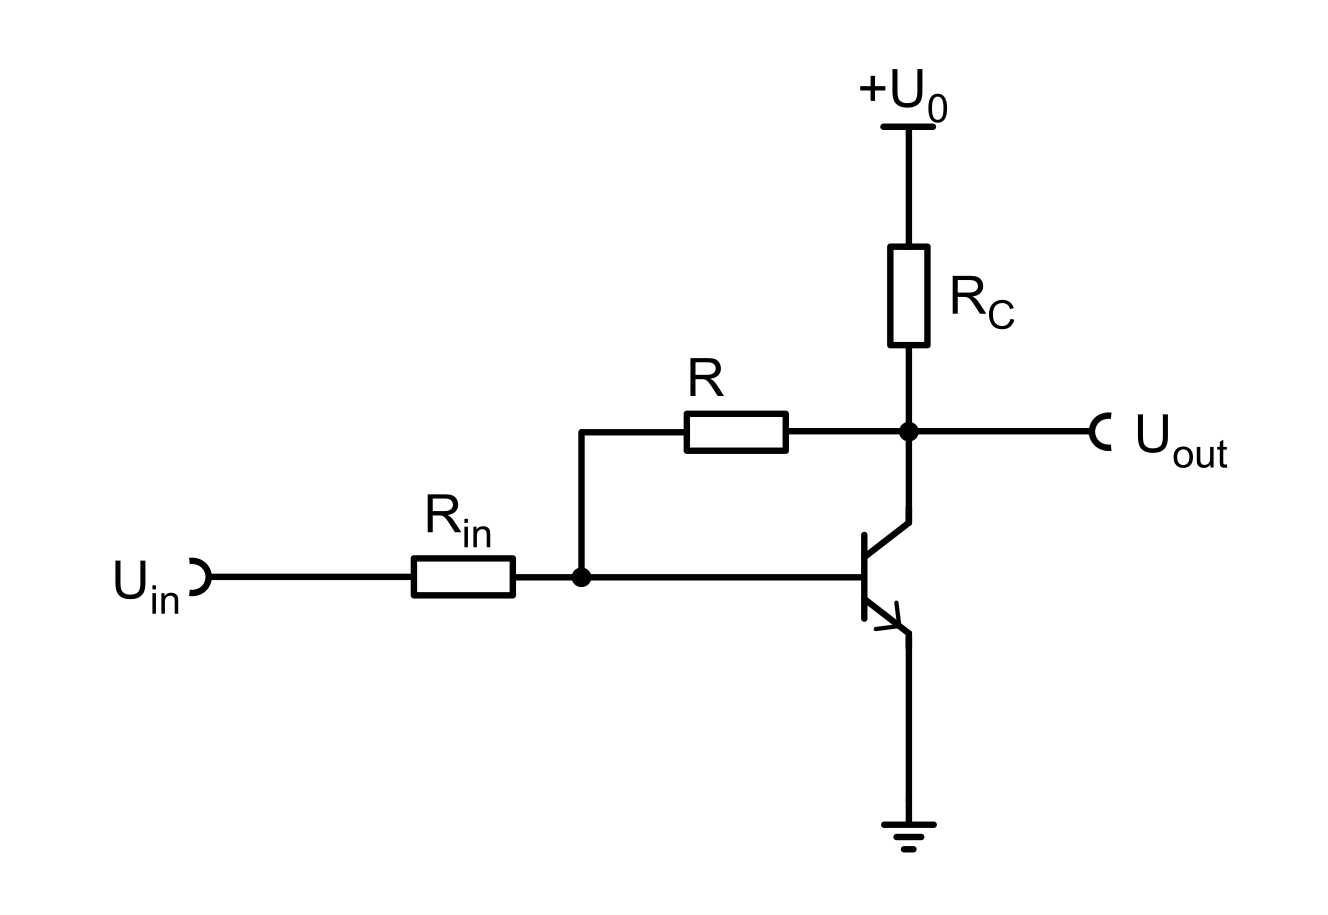
\includegraphics[width=0.6\textwidth]{spannungsgegenkopplung.png}
                \captionof{figure}{Transistor amplifier as common collector with negative feedback (voltage); figure 3/4.16 \cite{Praktikumsanleitung}}
        \end{Figure}
        In this figure the resistor $R$ sets the base potential as well as the operating point and cupples the voltage from the collector back to the base.
        Due to this negative feedback the base current is reduced although the input current remains constant.

	\newpage
	\section{Preliminary Tasks}
	\subsection{G}
	$\zz\ \nu =\tfrac{\gamma R_E}{r_{BE}+\gamma R_E}$ with $\gamma =\diff[]{I_E}{I_B}$ and $r_{BE}=\diff[]{U_{BE}}{I_B}$.
	\begin{align}
		                &  & \nu  & = \diff[]{U_E}{U_B}                                                    &  &           \\
		\Leftrightarrow &  &   & = \dfrac{\td I_ER_E}{\td U_{BE}+\td U_E}                               &  & \nonumber \\
		\Leftrightarrow &  &   & = \dfrac{\diff[]{I_ER_E}{I_B}}{\diff[]{U_{BE}}{I_B}+\diff[]{U_E}{I_B}} &  & \nonumber \\
		\Leftrightarrow &  &   & = \dfrac{\gamma R_E}{r_{BE}+\gamma R_E}.                               &  &
	\end{align}

	\subsection{H}
        The equation applies
	\begin{align}
		                &  & \dfrac{r_\text{out}}{r_\text{in}} & = \dfrac{\diff[]{U_E}{I_E}}{\diff[]{U_B}{I_B}} &  &           \\
		\Leftrightarrow &  &                                   & = \diff[]{U_E}{I_E}\diff[]{I_B}{U_B}           &  & \nonumber \\
		\Leftrightarrow &  &                                   & = \diff[]{U_E}{U_B}\diff[]{I_B}{I_E}           &  & \nonumber \\
		\Leftrightarrow &  &                                   & \approx 1\cdot \dfrac{1}{\gamma }.             &  &
	\end{align}

	\subsection{I}
        The equation applies
	\begin{align}
		                &  & \nu  & = \diff[]{U_C}{U_B}                                                    &  &           \\
		\Leftrightarrow &  &   & = \dfrac{\td I_CR_C}{\td U_{BE}+\td U_E}                               &  & \nonumber \\
		\Leftrightarrow &  &   & = \dfrac{\diff[]{I_CR_C}{I_B}}{\diff[]{U_{BE}}{I_B}+\diff[]{U_E}{I_B}} &  & \nonumber \\
		\Leftrightarrow &  &   & = \dfrac{\beta R_C}{r_{BE}+\gamma R_E}.                                &  &
	\end{align}

	\subsection{J}
        The equation applies
	\begin{align}
		                &  & \dfrac{1}{\nu}     & = \tfrac{1+k\nu _0}{\nu _0}                   &  &           \\
		\Leftrightarrow &  & \nu                & = \dfrac{\nu_0}{1+k\nu_0}                   &  & \nonumber \\
		\Leftrightarrow &  & \diff[]{\nu}{\nu_0}  & = \dfrac{1}{\left(1+k\nu_0\right)^2}      &  & \nonumber \\
		\Leftrightarrow &  &                  & = \dfrac{\nu}{\nu_0}\dfrac{1}{1+k\nu_0}       &  & \nonumber \\
		\Leftrightarrow &  & \dfrac{\td \nu}{\nu} & = \dfrac{\td \nu_0}{\nu_0}\dfrac{1}{1+k\nu_0} &  & \nonumber \\
		\Leftrightarrow &  &                  & = \dfrac{\td \nu_0}{\nu_0}\dfrac{\nu}{\nu_0}.   &  &
	\end{align}

	\subsection{K}
        The parallel capacitor with capacitance $C_{CB}$ and transistor form a high--pass filter.
        This means that high frequency signals will run through the capacitor and not the transistor, resulting in them not being amplified.

	\subsection{L}
        There is no voltage change at point P, because the input signal to the transistor T2 is constant.
        The change in current $\td I_E\left(T_2\right)$ is in return also zero.

	\subsection{M}
        For any transit frequency the equation holds $f_\text{grenz gk}\nu\left(f=0\right)=f_\text{grenz}\nu_0$.
	Thus $f_\text{grenz gk}=f_\text{grenz}\tfrac{\nu_0}{\nu\left(f=0\right)}$.

	\subsection{N}
        For increasing base current $I_B$, the collector voltage $U_C$ and the voltage across the resistor $U_{R_C}$ also increases.
        Because $U_0$ should be constant, the voltage drops across the resistor $R$, which in turn stabilizes the operating point.

	\clearpage
	\section{Analysis}
	\subsection{Voltageamplifier of the common collector}
	On Circut Board I (Fig. \ref{fig:cb1}) we construct a common collector with d$U_B=\SI{2.1}{V_{PP}}$ and $U_B\approx \SI{2}{V}$. To test the voltage ampilification we chose a variety of diffrent resistor combinations. The messurements are displayed in Tab. \ref{tab:voltage_amplification}. We expect no change for diffrent $R_E$.
	\begin{Figure}
		\centering
		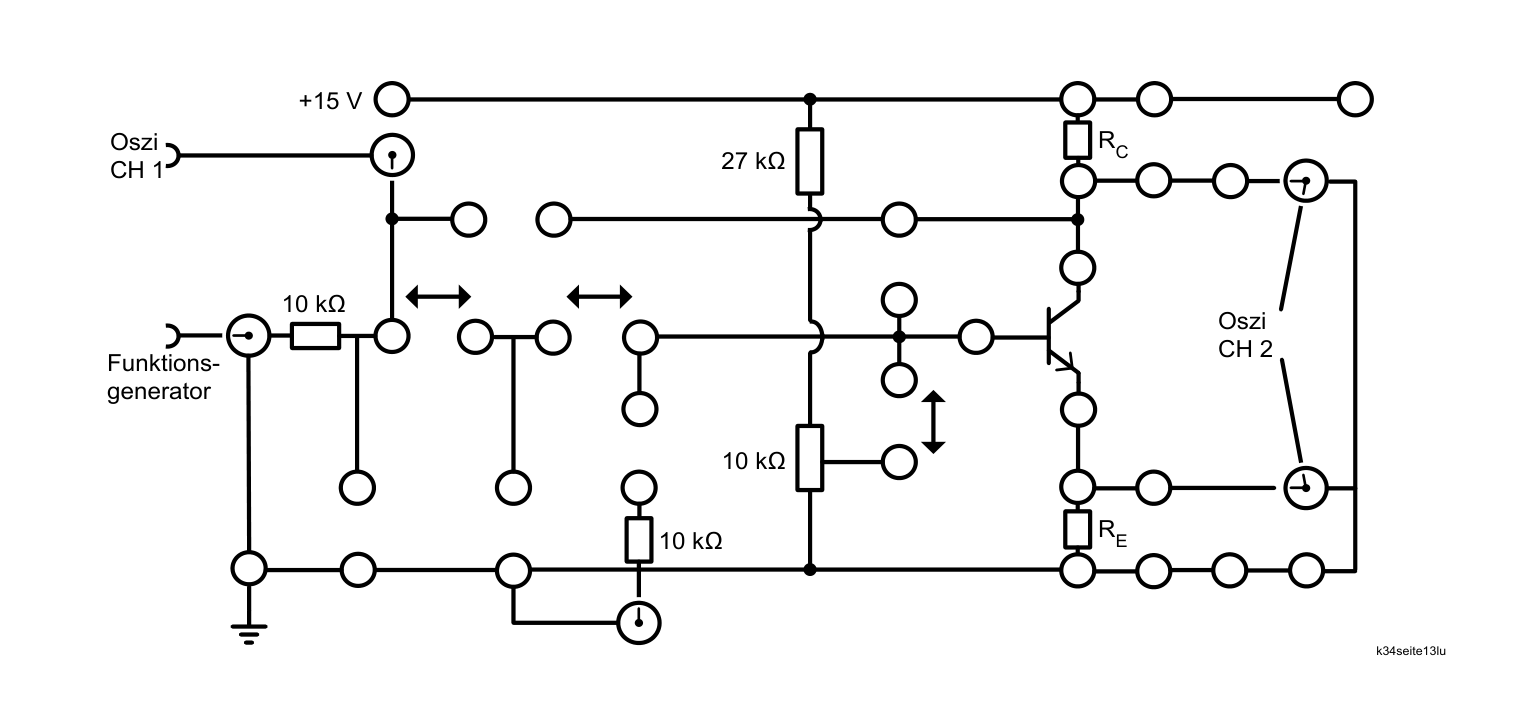
\includegraphics[width=1\textwidth]{circut_board_1.png}
		\captionof{figure}{Circut Board 1\cite{Praktikumsanleitung}}
		\label{fig:cb1}
	\end{Figure}
	\begin{center}
		\begin{tabular}{|c|c|c|}
			\hline
			$R_C$            & $R_E$            & amplification $\nu$    \\
			\hline
      \SI{360}{\Omega} & \SI{1}{k\Omega}  & \SI{1+-0.025}{}     \\
      \SI{360}{\Omega} & \SI{22}{k\Omega} & \SI{1.025+-0.025}{} \\
      \SI{360}{\Omega} & \SI{47}{k\Omega} & \SI{1.015+-0.025}{} \\
			\hline
      \SI{1}{k\Omega}  & \SI{360}{\Omega} & \SI{0.945+-0.025}{} \\
      \SI{22}{k\Omega} & \SI{360}{\Omega} & \SI{0.114+-0.025}{} \\
      \SI{47}{k\Omega} & \SI{360}{\Omega} & \SI{0.12+-0.025}{}  \\
			\hline
		\end{tabular}
		\captionof{table}{Voltage amplification for diffrent resistor combinations}
		\label{tab:voltage_amplification}
	\end{center}
        As we see, there is no significant variation of the amplification for diffrent $R_E$. Though we can clearly see a lowering of the amplification for higher $R_C$, wich is plausible since we have less current that can be amplified.

        \subsection{Common Collector as Buffer Amplifier}
        Here we are tasked to match the impedance of a speaker, so we are able to hear an output. For this we firstly construct an Inverted Amplifiert and test the speaker solely without a Common Collector. We observe, that the speaker does not produce any sound, because we havent matched the impedance. Now we add a Common Collecter as a Buffer Amplifier, wich in theroy should be able to match the impedance of the speaker. Unfortunatly we could not get the circut running and test the hypothisis. 
        \subsection{Inverted Amplifier}
        \subsubsection{Phasere Relationship between input and output}
        Now we build a Common Emitter on Circut Board I 

        \subsection{Alternating current cancellation of negative feedback}
        In this task, the noise visible on the oszillograph is reduced by increasing the voltage of the input signal.
        \\\\Changing $R_E$ to be zero, the amplification $|\nu |$ is maximised.
        The range in which the transistor has enough voltage to output a sinusoidal signal, meaning the signal lies within the dynamic range, is between $R_P  \in  \left[\SI{1.359}{k\ohm},\SI{3.161}{k\ohm}\right]$.
        $R_P$ is the potentiometer changing the offset voltage.
        For $R_E=\SI{390}{\ohm}$ (which is $|\nu |=1$), the potentiometer has a range of $R_P  \in  \left[\SI{1.178}{k\ohm},\SI{10}{k\ohm}=\text{max}\left(R_P\right)\right]$.
        \\\\Now a capacitor with capacitance $C=\SI{0.1}{\micro F}$ is connected in parallel with $R_E$.
        The previous amplification of around $10$ is achieved for a signal with frequency $\SI{44}{kHz}$.
        This makes sense, because the capacitor in parallel acts as a low pass, letting frequencies below $\SI{44}{kHz}$ pass through it, such that no amplification of 10 is achieved.
        The resistance above $\SI{44}{kHz}$ is high enough so that the signal passes through the transistor and gets amplified.

        \subsection{Frequency response of a cascode circuit}
        A \hyperref[fig:transistorverstärker]{transistor amplifier circuit} is constructed on \hyperref[fig:schaltbrett_2]{circuit board 2}.
        Output 2 is used here.
        \begin{Figure}
                \centering
                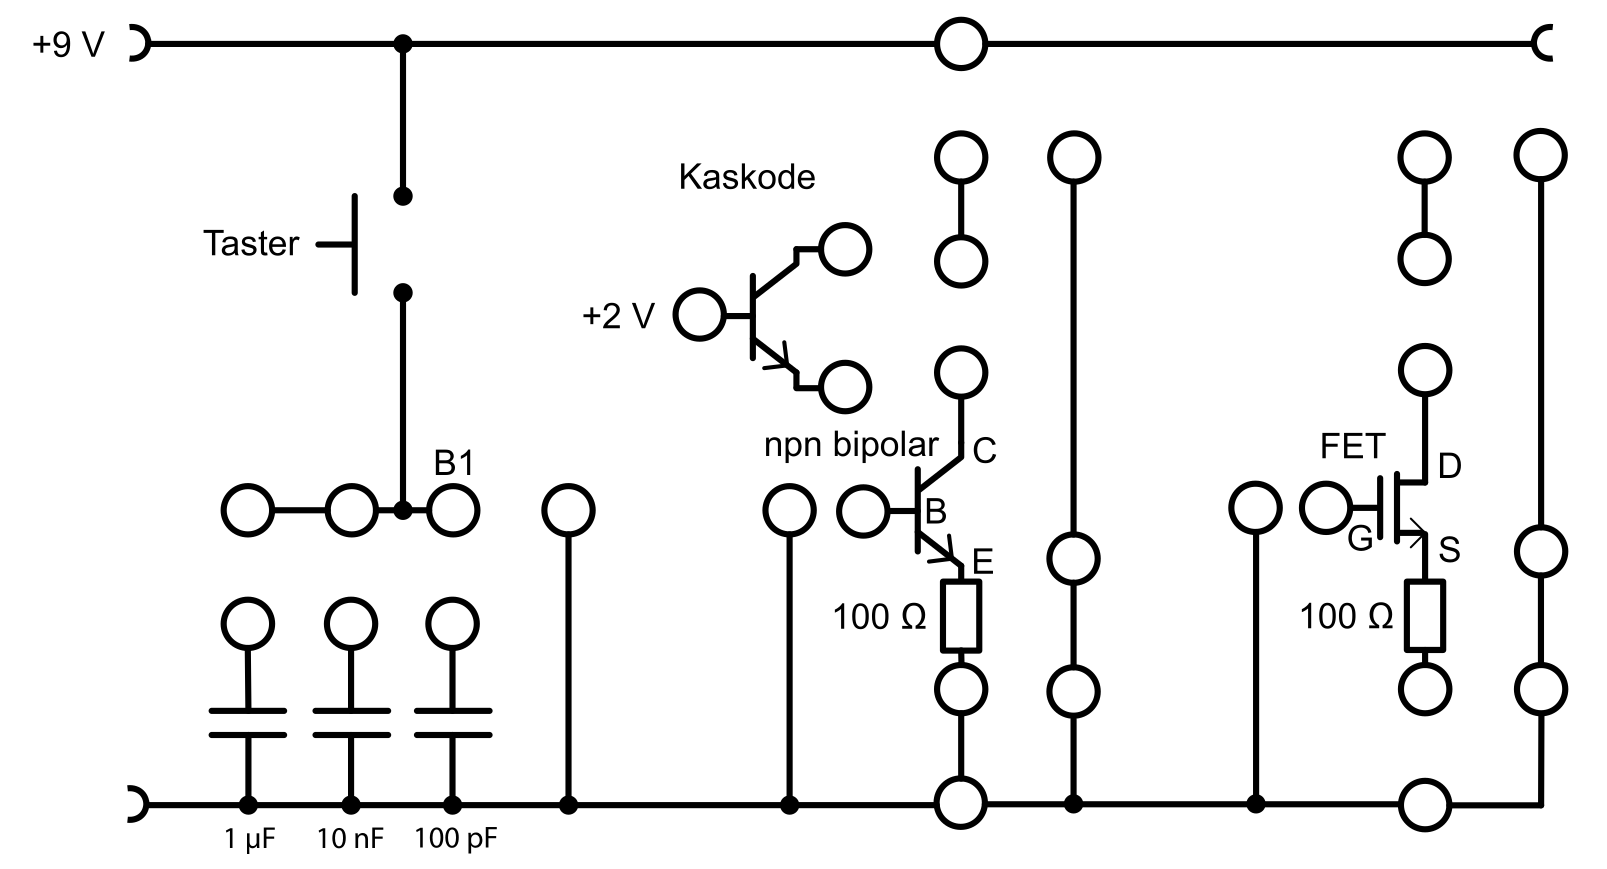
\includegraphics[width=0.6\textwidth]{schaltbrett_2.png}
                \captionof{figure}{Circuit board 2; Abb. 3.5\cite{Praktikumsanleitung}} \label{fig:schaltbrett_2}
        \end{Figure}
        \begin{Figure}
                \centering
                \includegraphics[width=0.6\textwidth]{transistorverstärker.png}
                \captionof{figure}{Transistor amplifier circuit using output 2; Abb. 3/4.15\cite{Praktikumsanleitung}} \label{fig:transistorverstärker}
        \end{Figure}
        To achieve an amplification of 10, the emitter and collector resistors are chosen to be $R_E=\SI{100}{\ohm}$ and $R_C=\SI{1}{k\ohm}=10\cdot R_E$.
        The input signal is a sinusoidal wave of $\SI{100}{Hz}$ with $U_{PP}=\SI{100}{mV}$.
        The DC--offset is set via a voltage divider.

\end{multicols}

\clearpage
\listoffigures
\listoftables
\bibliographystyle{plain}
\bibliography{refs}

%}}}

\end{document}
